\chapter{Experimentos.}\label{cap.experimentos}
\hspace{1cm} En este cap\'itulo se van a comentar los distintos experimentos realizados tanto con el drone real como en la simulaci\'on. Dado que el algoritmo consta de 3 fases principales (despegue, busqueda y aterrizaje), se va a comentar cada una de estas por separado, en simulaci\'on y con el robot real, para terminar comentando un caso del algoritmo completo. 

\section{Despegue en la simulaci\'on}
\hspace{1cm} Este es el mas sencillo de todos debido a que el drone en el Gazebo no tiene deriva y despega totalmente en vertical. Sobre esta parte se hicieron muchas pruebas de la parte perceptiva, pues al despegar sobre la baliza se observaba si detectaba bien los distintos colores de \'esta. En la parte de control las velocidades que se le daban al drone eran muy peque~nas, para que este se centrara ya que en el despegue pod\'ia estar sobre la baliza pero no totalmente centrado. 
\hspace{1cm} Se realiz\'o una prueba en la que el drone se situaba sobre un coche que tenia una baliza mientras \'este se desplazaba, de forma que el drone se moviera a la vez que lo hacia el coche. 
\hspace{1cm} Para finalizar, se realizo un control de banda muerta, en el que si el drone estaba descentrado por una peque~na distancia lo tratara igual que si estuviera totalmente en el centro. Esto se hizo para evitar peque~nos tambaleos cuando estuviera pr\'acticamente centrado. 


\begin{figure}[H]
	\centering
		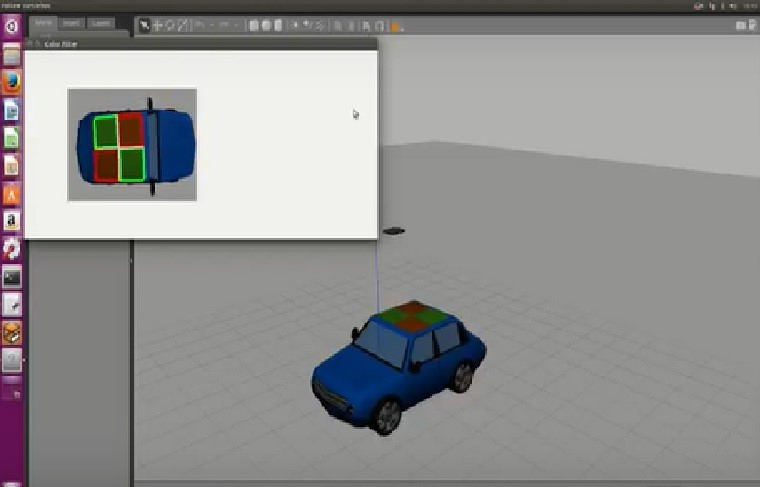
\includegraphics[width=0.8\textwidth]{imgs/TakeOff.jpg}
	\label{fig:Despegue sobre la baliza del coche.}
\end{figure}

\section{Despegue en el drone real}
\hspace{1cm} Para la realizaci\'on de este experimento situ\'abamos la baliza real sobre el suelo y el drone sobre esta, y as\'i al despegar ten\'ia un punto sobre el que centrarse. Esta parte se decidi\'o implementar porque el drone ten\'ia una deriva que le llevaba a desplazarse hacia atr\'as cuando ten\'ia que estar en el sitio. Cuando se hicieron las primeras pruebas de esto, se vi\'o que el drone siempre despegaba en esta direcci\'on y hab\'ia un dos segundos en los que no se pueden controlar sus movimientos, por tanto hab\'ia que contar con este desplazamiento. Destacar que en este punto la parte de percepci\'on era correcta, pues al pasar por encima de la baliza se observaba como detectaba los cuadrados de esta y el centro, donde se formaba la cruceta. Sin embargo, en la parte de control ten\'ia mas fuerza la instrucci\'on del despegue que la que se le enviaba al drone, y por tanto no se ten\'ia el control. 

\begin{figure}[H]
 \centering
  \subfloat[Despegue vista baliza]{
   \label{f:Vista baliza}
    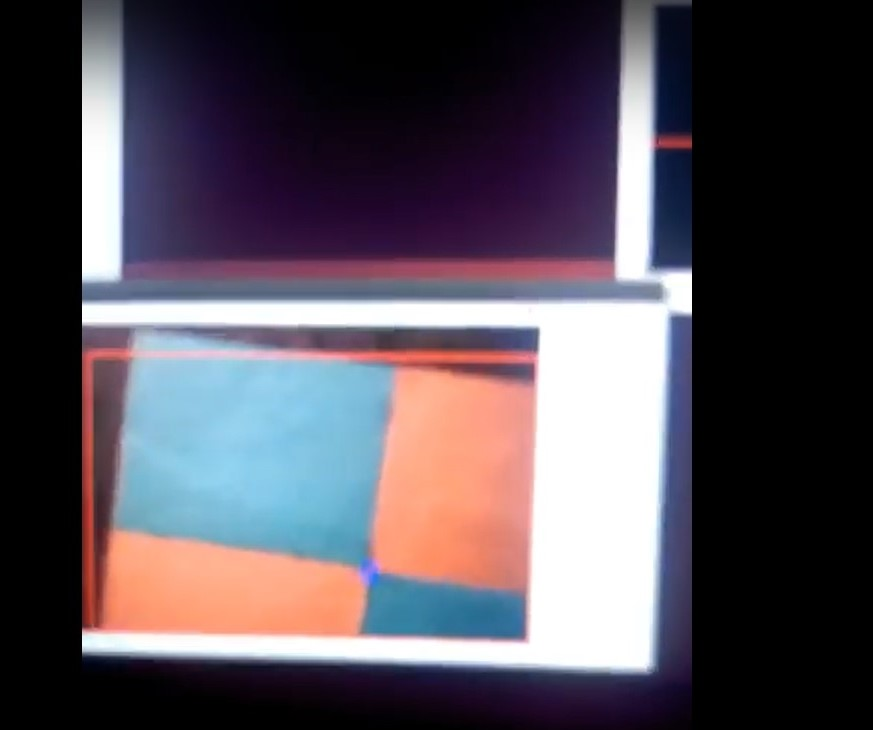
\includegraphics[width=0.4\textwidth]{imgs/takeoff_baliza.jpg}}
  \subfloat[Despegue vista drone]{
   \label{f:Drone}
    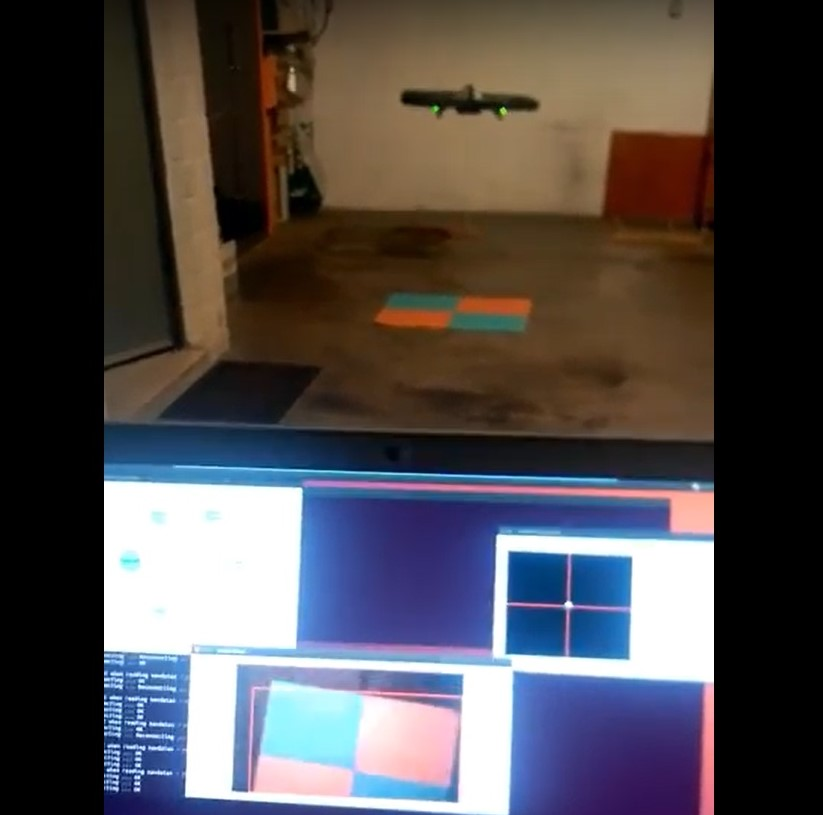
\includegraphics[width=0.4\textwidth]{imgs/takeoff_baliza2.jpg}}
 \caption{Despegue}
 \label{f:Test Despegue}
\end{figure}

\section{B\'usqueda en el simulador}
\hspace{1cm} Para la realizaci\'on de \'esta parte del algoritmo, como ya he comentado anteriormente, el drone va movi\'endose en espiral hasta encontrar la baliza, para ya centrarse sobre esta. Al principio de los experimentos, el drone se situaba cerca de la baliza para empezar su desplazamiento y que al encontrar la baliza se centrara. Una vez esto funcionaba, se probaba a poner el drone m\'as lejos de \'esta para que en la primera vuelta de la espiral no encontrara ning\'un objeto de inter\'es, pero ya en la segunda vuelta pudiera verlo y se centrara, comprobando de esta forma que las espirales se realizaban de forma correcta. La parte de percepci\'on era la correcta, pues el tratamiento de im\'agenes era igual al anterior, pero en la parte de control se pod\'ia observar el cambio de velocidad que se daba en el momento que estaba buscando y le aparec\'ia un objeto de inter\'es, por lo que se hicieron distintas pruebas modificando las velocidades y los cambios de una parte a otra del algoritmo, evitando as\'i los movimientos bruscos y los posibles problemas que pod\'ia dar esto en el drone real. 

\begin{figure}[H]
	\centering
		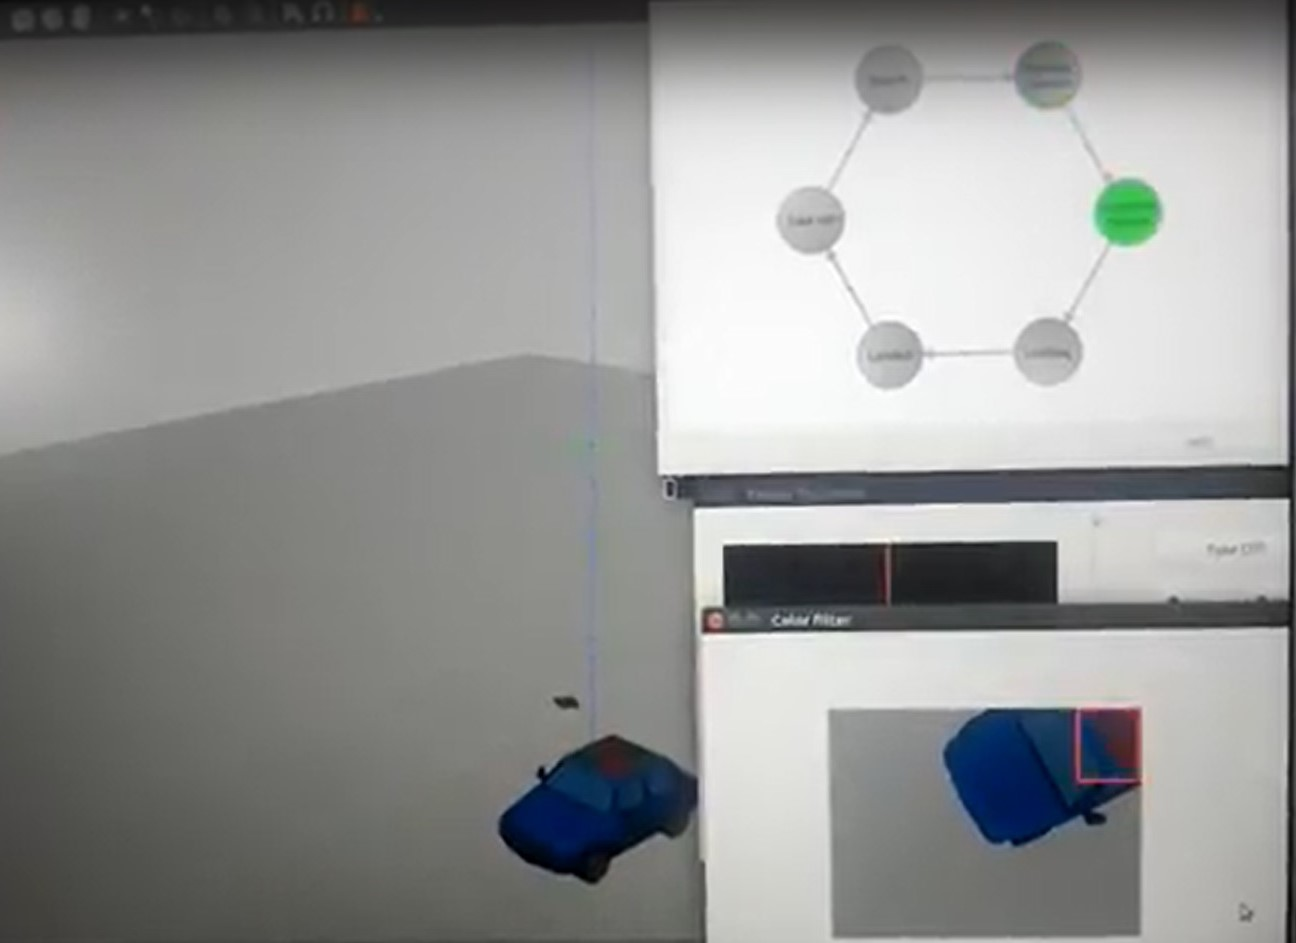
\includegraphics[width=0.8\textwidth]{imgs/search_simulate.jpg}
	\label{fig:Despegue sobre la baliza del coche.}
\end{figure}

\section{B\'usqueda en el drone real}
\hspace{1cm} Los experimentos en \'esta parte pueden dividirse totalmente en la parte de percepci\'on y en la parte de control. Lo primero que se probo fue que el algoritmo se moviera por un espacio grande realizando espirales, y ver que hac\'ia estas correctamente. Una vez se vio \'esto, se puso la baliza en el suelo y comenz\'o el algoritmo de busqueda, y una vez que detectara el objeto se le mandaba la orden de aterrizar. Una vez se vio que las dos partes funcionaban correctamente, ya se prob\'o que el drone se centrara sobre la baliza una vez la detectara, probando de esta forma el control sobre el drone real, viendo que no se realizaban movimientos bruscos con el controlador programado. Destacar que para las pruebas en espacios peque~nos, el algoritmo de b\'usqueda se cambi\'o, y en lugar de realizar espirales, el drone se mov\'ia realizando cuadrados, de forma que se ten\'ia un movimiento mas controlado y evitar posibles accidentes. 
\begin{figure}[H]
	\centering
		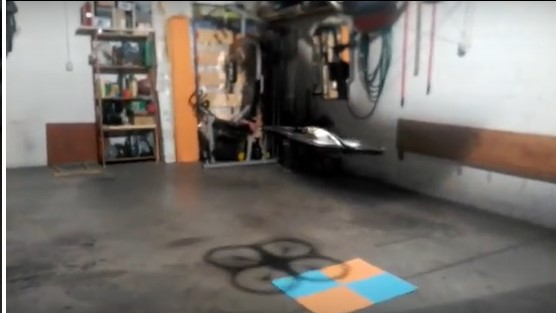
\includegraphics[width=0.8\textwidth]{imgs/search_real.jpg}
	\label{fig:Despegue sobre la baliza del coche.}
\end{figure}

\section{Aterrizaje en el simulador}
\hspace{1cm} En los experimentos de esta parte, nos hemos centrado en la parte de control. Lo que se trat\'o fue que el drone se centrara sobre la baliza sin realizar movimientos bruscos, una vez que el drone detectaba que estaba pr\'acticamente centrado sobre la baliza, comenzaba a descender, y una vez detectaba que estaba lo suficientemente cerca enviaba la orden de aterrizar. Como podemos observar, en estos experimentos la parte de percepci\'on se basan en controlar el centro de la baliza y el \'area, para tener una aproximaci\'on de la distancia que hab\'ia a \'esta. 


\begin{figure}[H]
 \centering
  \subfloat[Aterrizando]{
   \label{f:Aterrizando}
    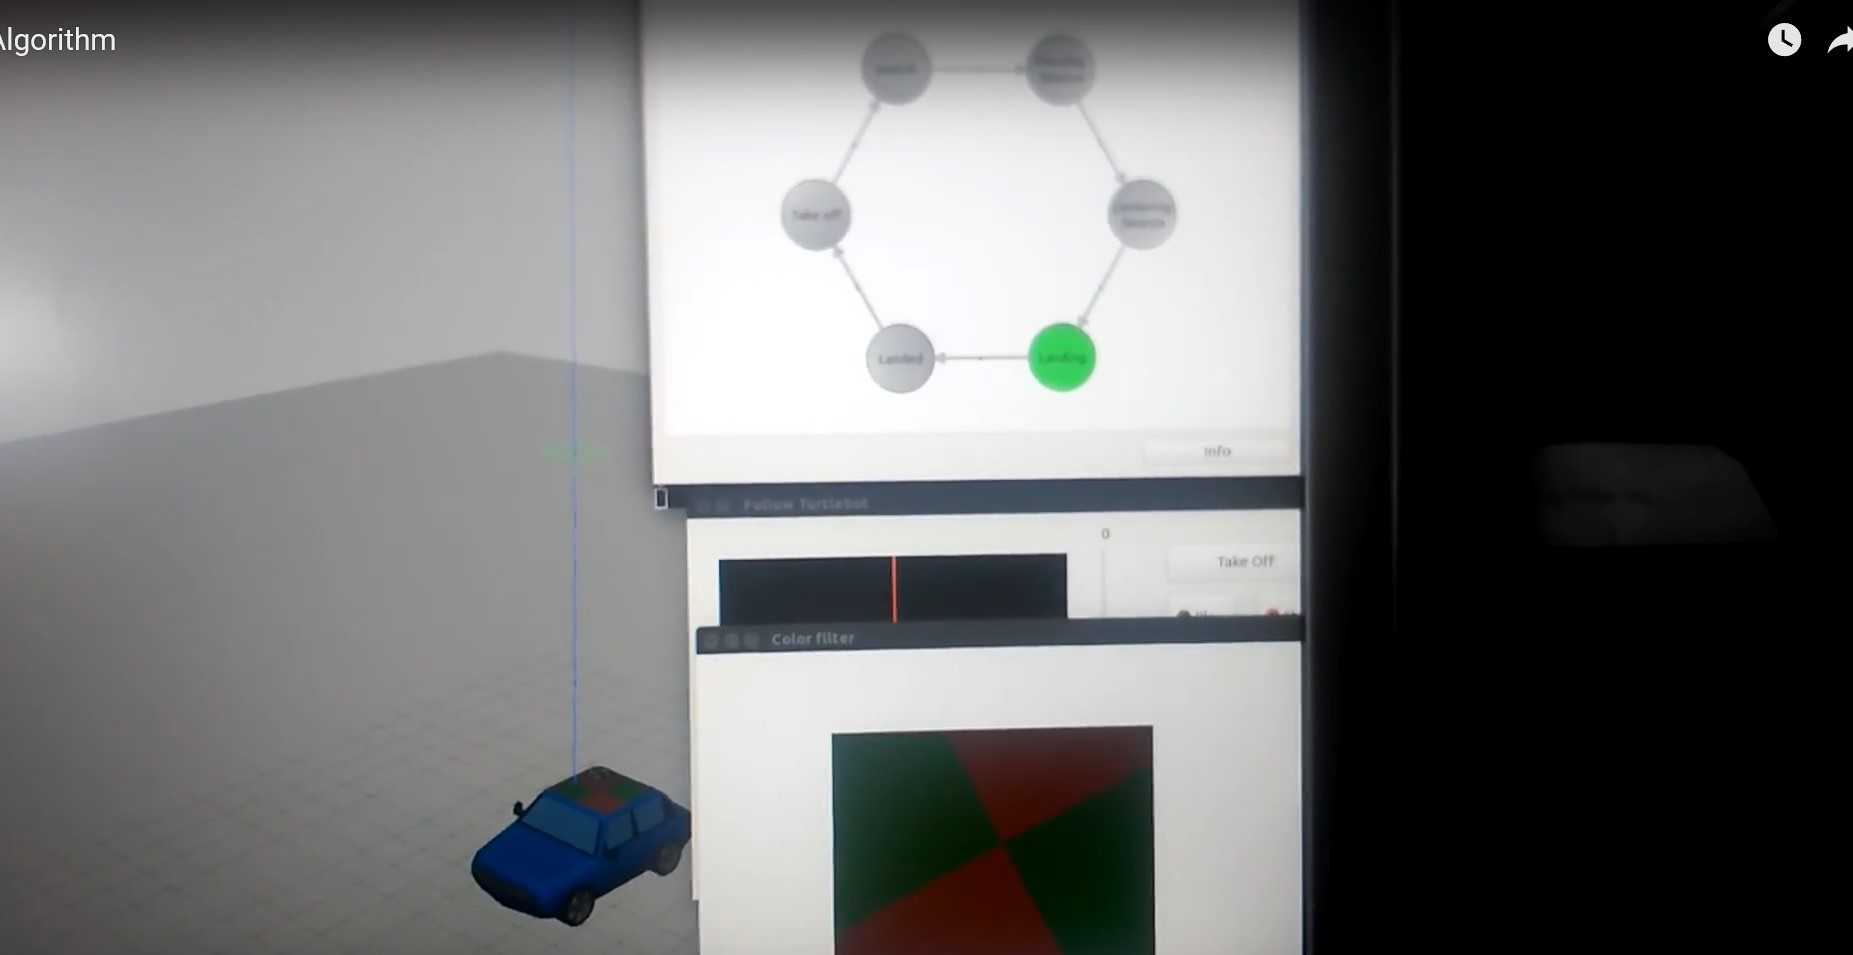
\includegraphics[width=0.4\textwidth]{imgs/landing.jpg}}
  \subfloat[Aterrizado]{
   \label{f:Aterrizado}
    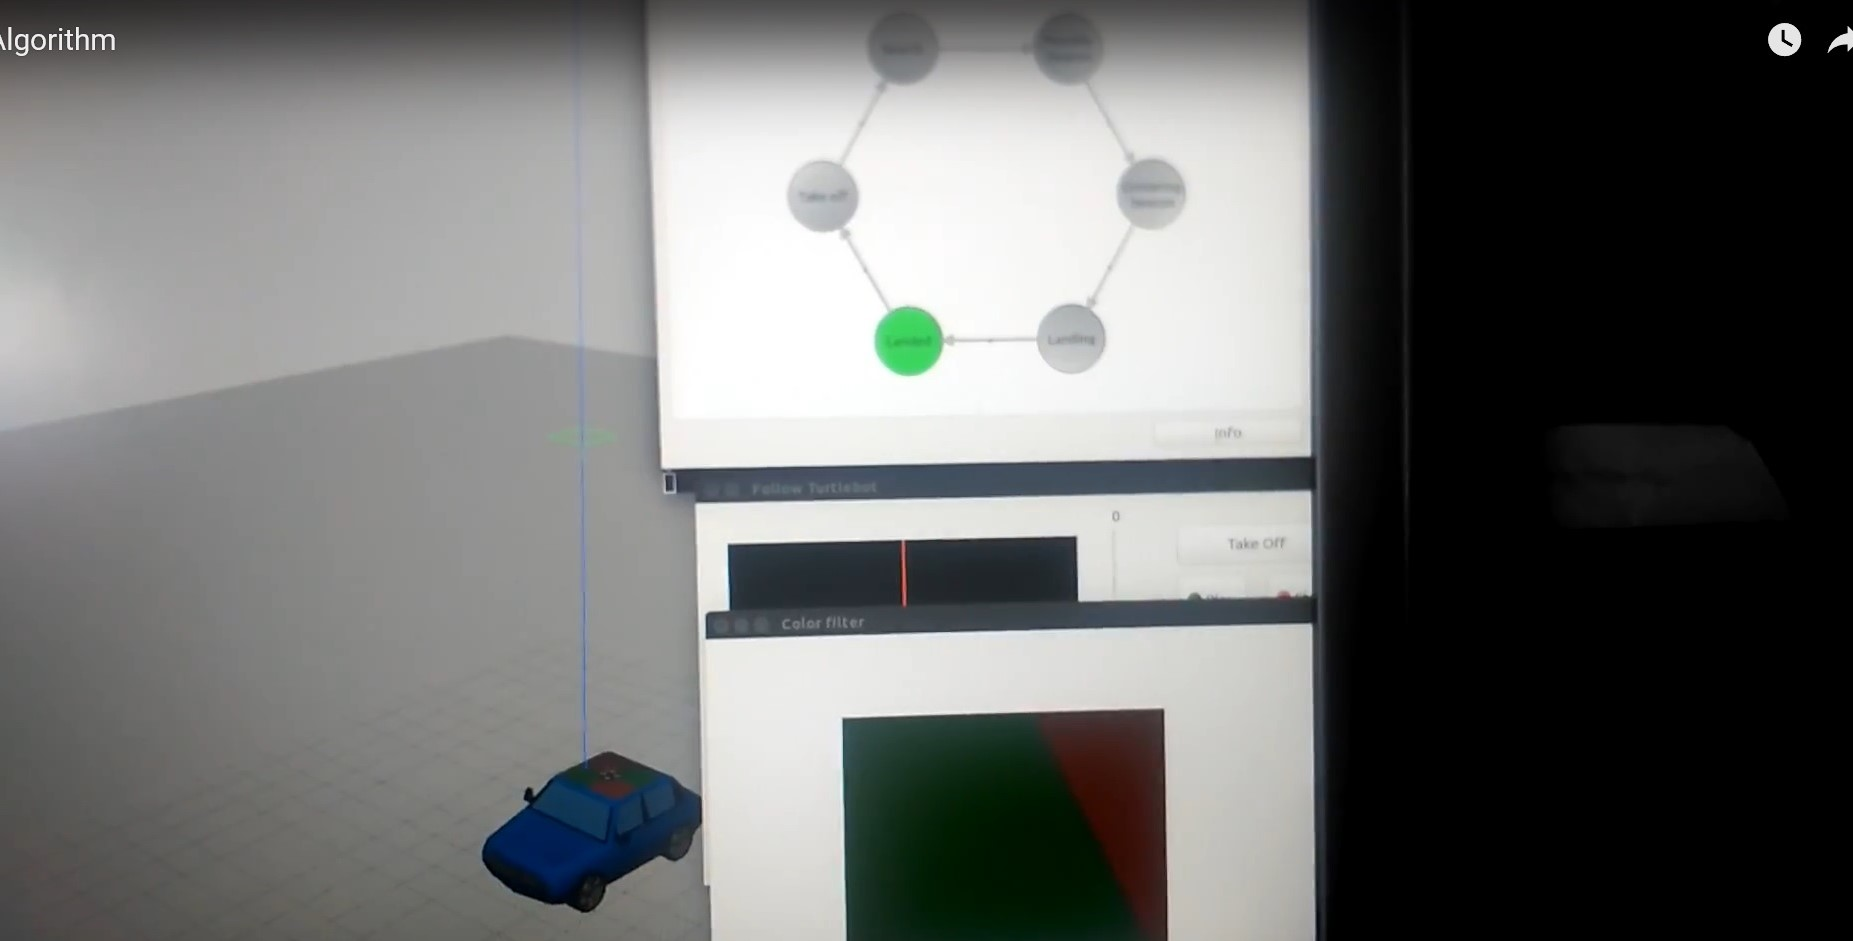
\includegraphics[width=0.4\textwidth]{imgs/landed.jpg}}
 \caption{Aterrizaje}
 \label{f:Test aterrizaje}
\end{figure}

\section{Aterrizaje en el drone real}
\hspace{1cm} Para la realizaci\'on de estos experimentos, teniendo la parte de percepci\'on anteriormente desarrollada, las primeras pruebas de control se realizar\'on de forma que, una vez el drone encontraba la baliza, aterrizara. En estas pruebas se obten\'ian buenos resultados, pero el drone no aterrizaba sobre la baliza ya que tra\'ia una velocidad en determinado sentido de la busqueda, y por lo tanto, el aterrizaje no era totalmente vertical sino que continuaba en este sentido. Tras esto, se hizo la prueba centrando el drone tras la busqueda y una vez estuviera centrado ya aterrizara sobre la baliza, obteniendo as\'i un aterrizaje mas vertical y pos\'andose el drone sobre la baliza. 
\begin{figure}[H]
	\centering
		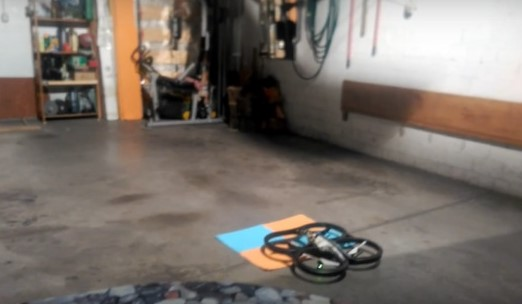
\includegraphics[width=0.4\textwidth]{imgs/landed_real.jpg}
	\label{fig:Aterrizaje sobre la baliza real.}
\end{figure}


\section{Algoritmo completo en el simulador}
\hspace{1cm} Este experimento se realizo para comprobar que todo lo que se hab\'ia programado por partes funcionaba tambi\'en si se probaba el algoritmo completo. Cabe destacar que las pruebas salieron correctamente. Sobre el simulador se probo a poner el drone sobre la baliza, que despegaba y se situaba en el centro de esta. Una vez pasaron 10 segundos y el drone continuaba en el centro, se hizo que este se alejara y perdiera la referencia de la baliza, y comenzara su algoritmo de busqueda. Una vez realizaba las espirales, en el momento que detectaba los colores de la baliza se centraba sobre estos, y una vez estaba practicamente centrado, comenzaba a descender, hasta que detectaba que estaba a una altura suficiente y se le pod\'ia mandar la orden de aterrizar, pos\'andose as\'i sobre la baliza. 

\section{Algoritmo completo en el drone real}
\hspace{1cm} Para esta prueba, se colocaron dos puntos de referencia. Una baliza sobre la que situarse al despegar. De esta forma al comenzar el algoritmo, cuando detectaba esta baliza se centraba sobre \'esta, y una vez pasaron 10 segundos comenzaba el algoritmo de b\'usqueda. En esta parte el drone se iba desplazando en funci\'on de las ordenes que se le mandaban en cada momento, hasta el momento en el que encontraba la baliza, momento en el que se centraba sobre esta y se le mandaba la orden de aterrizaje, quedando de esta forma el drone sobre la baliza. 



